\documentclass{article}
\usepackage{amssymb}
\usepackage{amsmath}
\usepackage{graphicx}
\usepackage{subcaption}
\usepackage{xurl}
\title{\textbf{ECE 6560 Final Project - Image Smoothing}}
\author{Alexander Domagala}
\date{Spring 2024}

\begin{document}
  \maketitle

  %%%%%%%%%%%%%%%%%%%%%%%%%%%%%%%%%%%%%%%%%%%%%%%%%%%%%%%%%%%%%%%
  % Problem Description
  %%%%%%%%%%%%%%%%%%%%%%%%%%%%%%%%%%%%%%%%%%%%%%%%%%%%%%%%%%%%%%%
  \section{Problem Description}
  Although image processing techniques began to appear around the 1960s, the proliferation of inexpensive
  digital computing power has greatly widened the application pool. Image processing techniques
  can now be found in areas such as digital photography, medical imaging, and object detection/tracking.\\

  \noindent
  All these applications can be affected by a very common problem: image noise.
  Noise can render further processing ineffective, thus there exist a variety of approaches by which
  we can attempt to smooth and denoise images. More traditional denoising techniques
  may involve fixed convolutional kernels, eg. box blur, that indicate how a specific pixel
  can be updated as a weighted sum of its neighbors. Approaches of this nature can reduce the noise in
  exchange for the image appearing blurred.\\

  \noindent
  We can instead leverage PDEs to describe how an image should be updated depending on its local characteristics.
  Approaches that leverage PDEs offer noise reduction while also lessening the blurring that is done to edges.\\

  \noindent
  In this project, we will explore how we can tailor a PDE-based filter to suit a specific image.
  The goal is that by understanding the characteristics of the image's edges and noise, we
  will be able to outperform a more generalized PDE-based filter. Our filter will be developed
  using techniques falling under Anisotropic Diffusion.




  %%%%%%%%%%%%%%%%%%%%%%%%%%%%%%%%%%%%%%%%%%%%%%%%%%%%%%%%%%%%%%%
  % Mathematical Modeling
  %%%%%%%%%%%%%%%%%%%%%%%%%%%%%%%%%%%%%%%%%%%%%%%%%%%%%%%%%%%%%%%
  \newpage
  \section{Mathematical Modeling}

  %%%%%%%%%%%%%%%%%%%%%%%%%%%%%%
  % Introduction
  %%%%%%%%%%%%%%%%%%%%%%%%%%%%%%
  \subsection{Introduction}
  Before explicitly developing our PDE, we must first understand the behavior that we want our system to have.
  We will leverage the Calculus of Variations. This is a powerful framework that will help us arrive at a PDE
  that reflects some desired behavior. Examine the following equation
  \begin{center}
    \begin{tabular}{l}
      $E(I) = \int_{0}^{1} \int_{0}^{1} L(I, I_{x}, I_{y}, x, y) dx dy$
    \end{tabular}
  \end{center}

  \noindent
  $E(I)$ is the energy functional. Similar to the common understanding of a function, it can output
  a single value. The key difference is that the input to the energy functional, is another entire
  function that will depend on traditional variables like $x,y$, etc.\\

  \noindent
  Note that all notation before section (4) is for continuous space: $x,y \in \mathbb{R}$. Thus,
  the input to the energy functional can be thought of as an image with an infinite amount of pixels: $I(x,y)$.\\

  \noindent
  During lecture, the following example was introduced. If we want to measure how noisy a certain image is,
  we could measure the average value of the image's magnitude gradient squared.
  \begin{center}
    \begin{tabular}{l}
      $E(I) = \int_{0}^{1} \int_{0}^{1} \frac{1}{2} (\| \nabla_{I} \|)^{2} dx$
    \end{tabular}
  \end{center}

  \noindent
  Given two copies of the same image with different amounts of noise, the noiser image will have larger values
  for $E(I)$ while smoother image will have a smaller values for $E(I)$. The Calculus of Variations says
  that we can utilize the Euler Lagrange equation
  $L_{I} - \frac{\partial}{\partial x}L_{I_{x}} - \frac{\partial}{\partial y}L_{I_{y}} = 0$ to solve an
  optimization problem that minimizes the energy functional $E(I)$. Since we defined the
  energy functional to measure the average gradient squared, minimization will yield a method
  by which we can most efficiently reduce this criterion.\\

  \newpage
  \noindent
  In the case of the example, minimization yields the Linear Heat equation
  \begin{center}
    $I_{t} = \Delta I$
  \end{center}
  The Linear Heat equation optimally reduces the average squared value of the gradient in an image.
  This means that areas of high gradient in the image will be aggresively smoothed. Hence, the edges (which
  are areas of higher gradient) are not very well preserved with this technique.
  \begin{center}
    Quadratic Penalty: $x^2$\\
    \vspace{12pt}
    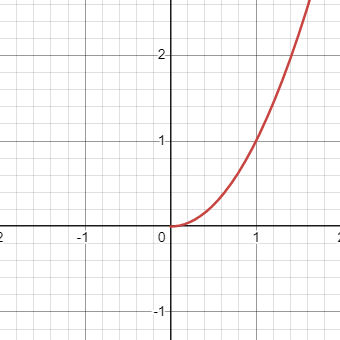
\includegraphics[scale=0.5]{../report_images/squared.png}
  \end{center}
  \vspace{12pt}

  \noindent
  A major improvement is to instead use a linear penalty. Smoothing that takes place at the edges
  will be less extreme than the previous case. This means that enough diffusion could take place
  in areas of low gradient such that the image appears to be denoised. Then, the diffusion can be stopped.
  Although the edges also experience diffusion, the penalty is much more lenient than the previous case.
  This method is known as Total Variation Diffusion.
  \begin{center}
    Linear Penalty: $x$\\
    \vspace{12pt}
    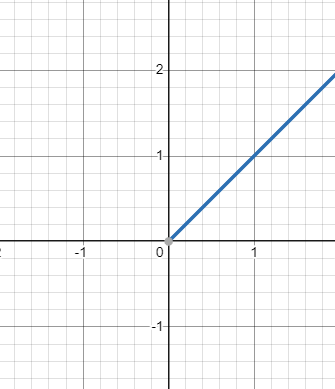
\includegraphics[scale=0.5]{../report_images/linear.png}
  \end{center}

  %%%%%%%%%%%%%%%%%%%%%%%%%%%%%%
  % Anisotropic Diffusion
  %%%%%%%%%%%%%%%%%%%%%%%%%%%%%%
  \newpage
  \noindent
  \subsection{Anisotropic Diffusion}
  The previous examples showed that by selecting a certain penalty and then minimizing the
  associated energy functional, we can control the smoothing behavior of a particular system.
  The examples can be generalized to what is known as Anisotropic or Perona-Malik Diffusion.
  We can continue towards the project goal of tailoring a penalty to a specific image
  by working under this framework.
  \begin{center}
    $E(I) = \iint C(\| \nabla_{I} \|) dx dy$
  \end{center}
  Note that the penalty $C(\| \nabla_{I} \|)$
  must be strictly increasing for the diffusion to be well-posed. We can
  arrive at our PDE via gradient descent\\

  \begin{center}
    \begin{tabular}{l}
      \vspace{12pt}
      $L(I,I_{x},I_{y},x,y) = C(\| \nabla_{I} \|)$\\
      \vspace{12pt}
      $L_{I} = 0$\\
      \vspace{12pt}
      $L_{I_{x}} = \dot{C}(\| \nabla_{I} \|) \frac{I_{x}}{\| \nabla_{I} \|}$\\
      \vspace{12pt}
      $L_{I_{y}} = \dot{C}(\| \nabla_{I} \|) \frac{I_{y}}{\| \nabla_{I} \|}$\\
      \vspace{12pt}
      $\nabla_{I}E = L_{I} - \frac{\partial}{\partial x}L_{I_{x}} - \frac{\partial}{\partial y}L_{I_{y}}$\\
      \vspace{12pt}
      $I_{t} = -\nabla_{I}E$\\
      \vspace{12pt}
      $I_{t} = -L_{I} + \frac{\partial}{\partial x}L_{I_{x}} + \frac{\partial}{\partial y}L_{I_{y}}$\\
      \vspace{12pt}
      $I_{t} = \frac{\partial}{\partial x}(\dot{C}(\| \nabla_{I} \|) \frac{I_{x}}{\| \nabla_{I} \|}) + \frac{\partial}{\partial y}(\dot{C}(\| \nabla_{I} \|) \frac{I_{y}}{\| \nabla_{I} \|})$\\
      \vspace{12pt}
      $I_{t} = \nabla \cdot (\frac {\dot{C}(\| \nabla_{I} \|)}{\| \nabla_{I} \|} \nabla I)$
    \end{tabular}
  \end{center}

  \noindent
  Now we will work to develop a custom penalty $C(\| \nabla_{I}\|)$ that supports
  enhanced edge preservation for a specific image.

  %%%%%%%%%%%%%%%%%%%%%%%%%%%%%%
  % Image Profiling
  %%%%%%%%%%%%%%%%%%%%%%%%%%%%%%
  \newpage
  \subsection{Image Profiling}
  Consider the following images
  \begin{figure}[!htb]
    \begin{center}
      \begin{subfigure}[b]{0.4\textwidth}
        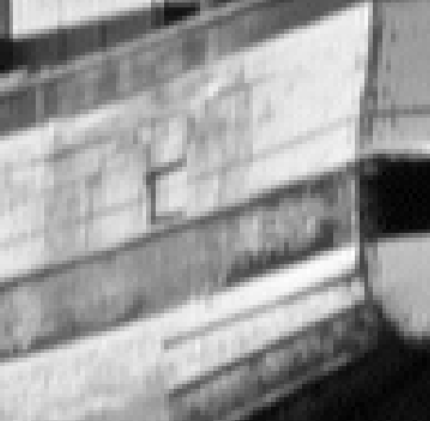
\includegraphics[width=\textwidth]{../report_images/boat_crop.png}
        \caption{Original Image}
      \end{subfigure}
      \hfill
      \begin{subfigure}[b]{0.4\textwidth}
        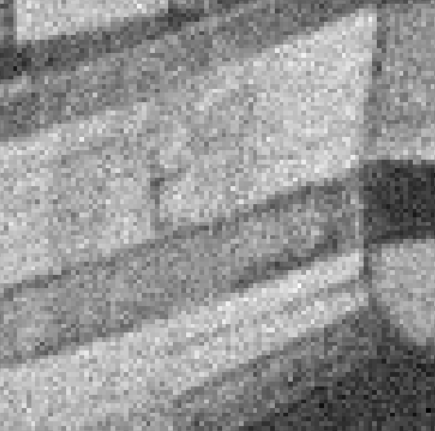
\includegraphics[width=\textwidth]{../report_images/noisy.png}
        \caption{Corrputed Image}
      \end{subfigure}
    \end{center}
  \end{figure}

  \noindent
  We can compute the magnitude gradient at each pixel in the images by using the following
  approximations. Note that, these are explained in further detail in section (4):
  \begin{center}
    \begin{tabular}{l}
      \vspace{12pt}
      $I_{x}(x,y,t) = \frac{I(x+\Delta x,y,t) - I(x-\Delta x,y,t)}{2\Delta x}$\\
      \vspace{12pt}
      $I_{y}(x,y,t) = \frac{I(x,y+\Delta y,t) - I(x,y-\Delta y,t)}{2\Delta y}$\\
      $\| \nabla_{I} \| = \sqrt{I_{x}^2 + I_{y}^2}$\\
    \end{tabular}
  \end{center}

  \noindent
  The following image shows the magnitude gradient at each pixel in the noisy image.
  Edges take on a lighter color while darker sections reflect more uniform areas of the image.
  \begin{center}
    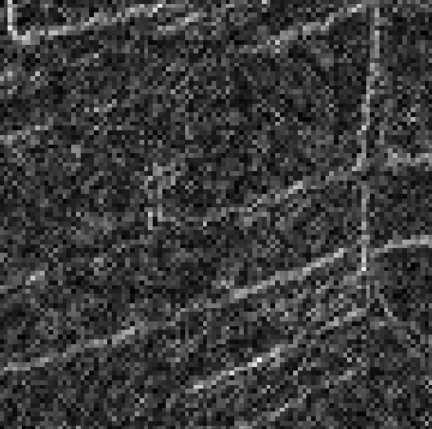
\includegraphics[scale=0.5]{../report_images/noisy_grad.png}
  \end{center}

  \newpage
  \noindent
  The distribution of the magnitude gradient can be visualized using a histogram.
  \begin{center}
    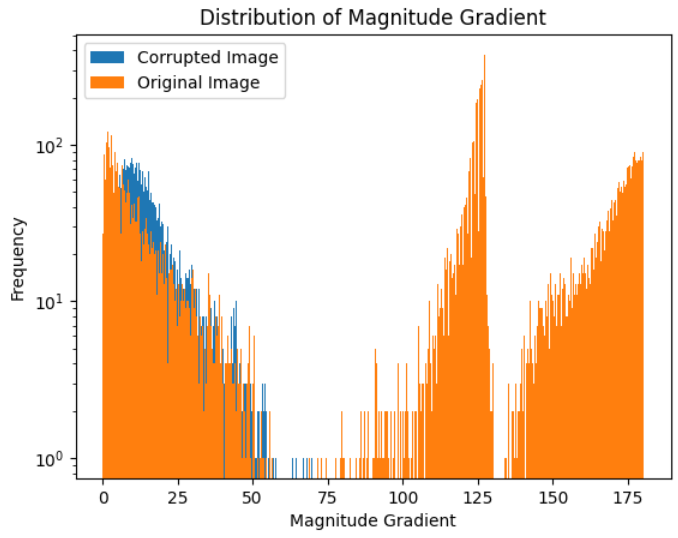
\includegraphics[scale=0.5]{../report_images/gradient.png}
  \end{center}
  \vspace{12pt}

  \noindent
  The corrputed image appears to differ in the range of 10 to 75.
  Let's shape the energy functional so that pixels in the image that
  fall in this range of gradients are smoothed. Thus, we
  can propose the following form for the penalty
  \begin{center}
    Sigmoidal Penalty: $\frac{\lambda}{1+e^{-(x-c)}}$\\
    \vspace{12pt}
    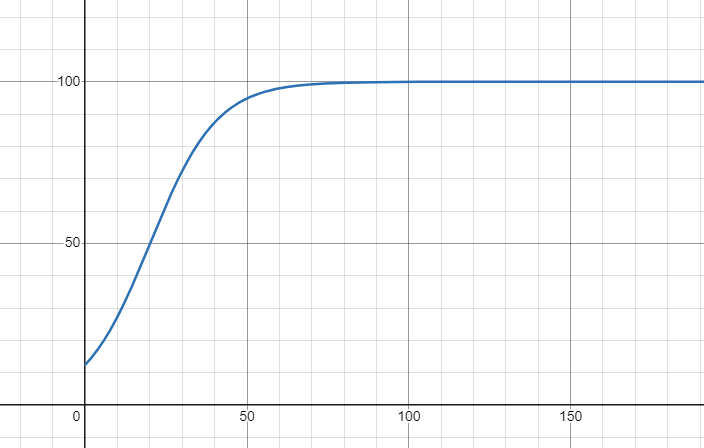
\includegraphics[scale=0.5]{../report_images/sigmoid.png}
  \end{center}
  \vspace{12pt}

  \noindent
  The goal of this penalty is to only have smoothing at the gradients
  that are corrputing the image. By keeping a nearly flat penalty in the for
  the higher gradients, we will greatly reduce the amount of diffusion that
  takes place along the edges.




  %%%%%%%%%%%%%%%%%%%%%%%%%%%%%%%%%%%%%%%%%%%%%%%%%%%%%%%%%%%%%%%
  % Derivation of PDE
  %%%%%%%%%%%%%%%%%%%%%%%%%%%%%%%%%%%%%%%%%%%%%%%%%%%%%%%%%%%%%%%
  \newpage
  \section{Derivation of PDE}

    \noindent Now, recall the Euler-Lagrange equation
      \begin{center}
        \begin{tabular}{l}
          \vspace{12pt}
          $L_{f} - \frac{\partial}{\partial x}L_{f'} = 0$ (1-D)\\
          $L_{I} - \frac{\partial}{\partial x}L_{I_{x}} - \frac{\partial}{\partial y}L_{I_{y}} = 0$ (2-D)\\
        \end{tabular}
      \end{center}
    \vspace{12pt}

    \noindent
    We can begin working towards obtaining our PDE by setting up a gradient descent
      \begin{center}
        \begin{tabular}{l}
          \vspace{12pt}
          $I_{t} = -\nabla_{I}E$\\
          $I_{t} = -L_{I} + \frac{\partial}{\partial x}L_{I_{x}} + \frac{\partial}{\partial y}L_{I_{y}}$
        \end{tabular}
      \end{center}
    \vspace{12pt}

    \noindent
    We will now have to compute terms $L_{I}$, $L_{I_{x}}$, $L_{I_{y}}$ using the previously obtained energy functional
      \begin{center}
        \begin{tabular}{l}
          $L(I,I_{x},I_{y},x,y) = \frac{\lambda}{1+e^{\alpha}}$, where $\alpha = -\frac{1}{\beta}(\| \nabla_{I} \|-c)$\\
          We will also include a term $\epsilon$ such that $\| \nabla_{I} \| = \sqrt{I_{x}^2 + I_{y}^2 + \epsilon^2}$\\
          $\epsilon$ is a constant used to prevent stability issues and will be examined more\\
          \vspace{12pt}
          closely in section (4).\\
          $L_{I} = \frac{\partial}{\partial I}(L)$\\
          $L_{I} = 0$\\
          $L_{I_{x}} = \frac{\partial}{\partial I_{x}}(L)$\\
          $L_{I_{x}} = \frac{\lambda}{\beta} \frac{e^\alpha}{(1+e^{\alpha})^2} \frac{I_{x}}{\sqrt{I_{x}^2 + I_{y}^2 + \epsilon^2}}$\\
          $L_{I_{y}} = \frac{\partial}{\partial I_{y}}(L)$\\
          $L_{I_{y}} = \frac{\lambda}{\beta} \frac{e^\alpha}{(1+e^{\alpha})^2} \frac{I_{y}}{\sqrt{I_{x}^2 + I_{y}^2 + \epsilon^2}}$\\
        \end{tabular}
      \end{center}
      \vspace{12pt}

    \noindent
    Now that we have obtained our expressions for $L_{I_{x}}$ and $L_{I_{y}}$, we must compute their partial derivatives
    as shown by the Euler-Lagrange equation. This will be shown for $\frac{\partial}{\partial x}L_{I_{x}}$. $\frac{\partial}{\partial y}L_{I_{y}}$ will be obtained by examining
    the expression of $\frac{\partial}{\partial x}L_{I_{x}}$.\\

    \noindent
    Let $\phi$ denote $\frac{e^\alpha}{(1+e^{\alpha})^2}$ and let $\gamma$ denote $\frac{I_{x}}{\sqrt{I_{x}^2 + I_{y}^2 + \epsilon^2}}$.
    We can begin finding $\frac{\partial}{\partial x}L_{I_{x}}$ by using the product-rule $\frac{\partial}{\partial x}(\gamma)\phi + \frac{\partial}{\partial x}(\phi)\gamma$.
    We will start with the left side of the sum. Note that we must include $\frac{\lambda}{\beta}$ in the final expression.\\
    \begin{center}
      \begin{tabular}{l}
        \vspace{12pt}
        $\frac{\partial}{\partial x}(\gamma)\phi$\\
        \vspace{12pt}
        $\frac{\partial}{\partial x}(\frac{I_{x}}{\sqrt{I_{x}^2 + I_{y}^2 + \epsilon^2}})\phi$\\
        $(\frac{I_{xx}}{(I_{x}^2 + I_{y}^2 + \epsilon^2)^\frac{1}{2}} - \frac{I_{x}}{(I_{x}^2 + I_{y}^2 + \epsilon^2)^\frac{3}{2}}(I_{x}I_{xx} + I_{y}I_{xy}))\phi$
      \end{tabular}
    \end{center}
    \vspace{12pt}
    
    \newpage
    \noindent
    We can now examine the right side of $\frac{\partial}{\partial x}(\gamma)\phi + \frac{\partial}{\partial x}(\phi)\gamma$.
    \begin{center}
      \begin{tabular}{l}
        $\frac{\partial}{\partial x}(\phi)\gamma$\\
        $\frac{\partial}{\partial x}(\frac{e^\alpha}{(1+e^{\alpha})^2})\gamma$\\
        $\frac{\partial}{\partial x}((e^\alpha)(1+e^{\alpha})^{-2})\gamma$\\
      \end{tabular}
    \end{center}

    \noindent
    We see that we will need to again perform the product-rule between $(e^\alpha)$ and\\
    $(1+e^{\alpha})^{-2}$. Taking the partial derivative of $(e^\alpha)$
    \begin{center}
      \begin{tabular}{l}
        $-\frac{1}{\beta} e^{\alpha} \frac{1}{(I_{x}^2 + I_{y}^2 + \epsilon^2)^\frac{1}{2}} (I_{x}I_{xx}+I_{y}I_{xy})$
      \end{tabular}
    \end{center}

    \noindent
    Taking the partial derivative of $(1+e^{\alpha})^{-2}$
    \begin{center}
      \begin{tabular}{l}
        $-2(1+e^{\alpha})^{-3} (-\frac{1}{\beta} e^{\alpha} \frac{1}{(I_{x}^2 + I_{y}^2 + \epsilon^2)^\frac{1}{2}} (I_{x}I_{xx}+I_{y}I_{xy})) $
      \end{tabular}
    \end{center}

    \noindent
    Thus, after factoring common terms, $\frac{\partial}{\partial x}((e^\alpha)(1+e^{\alpha})^{-2})$ yields
    \begin{center}
      \begin{tabular}{l}
        $[-\frac{1}{\beta} (e^\alpha) (\frac{1}{(I_{x}^2 + I_{y}^2 + \epsilon^2)^\frac{1}{2}}) (I_{x}I_{xx}+I_{y}I_{xy})] [(1+e^{\alpha})^{-2} + (e^\alpha)(-2(1+e^{\alpha})^{-3})]$\\
      \end{tabular}
    \end{center}
    \vspace{12pt}
    \vspace{12pt}

  \noindent
  We have reached the final expression for $\frac{\partial}{\partial x}L_{I_{x}}$
  \begin{center}
    \begin{tabular}{l}
      \vspace{12pt}
      $\frac{\partial}{\partial x}L_{I_{x}} =$\\
      \vspace{12pt}
      $\frac{\lambda}{\beta}[[ (\frac{I_{xx}}{(I_{x}^2 + I_{y}^2 + \epsilon^2)^\frac{1}{2}}) - (\frac{I_{x}}{(I_{x}^2 + I_{y}^2 + \epsilon^2)^\frac{3}{2}}) (I_{x}I_{xx} + I_{y}I_{xy})] (\frac{e^\alpha}{(1+e^{\alpha})^2}) +$\\
      \vspace{12pt}
      $(\frac{I_{x}}{(I_{x}^2 + I_{y}^2 + \epsilon^2)^\frac{1}{2}}) [-\frac{1}{\beta} (e^\alpha) (\frac{1}{(I_{x}^2 + I_{y}^2 + \epsilon^2)^\frac{1}{2}}) (I_{x}I_{xx}+I_{y}I_{xy})] [(1+e^{\alpha})^{-2} + (e^\alpha)(-2(1+e^{\alpha})^{-3})]]$
    \end{tabular}
  \end{center}
  \vspace{12pt}

  \noindent
    $\frac{\partial}{\partial y}L_{I_{y}}$ can be obtained by modifying $\frac{\partial}{\partial x}L_{I_{x}}$
    \begin{center}
      \begin{tabular}{l}
        \vspace{12pt}
        $\frac{\partial}{\partial y}L_{I_{y}} =$\\
        \vspace{12pt}
        $\frac{\lambda}{\beta}[[ (\frac{I_{yy}}{(I_{x}^2 + I_{y}^2 + \epsilon^2)^\frac{1}{2}}) - (\frac{I_{y}}{(I_{x}^2 + I_{y}^2 + \epsilon^2)^\frac{3}{2}}) (I_{x}I_{xy} + I_{y}I_{yy})] (\frac{e^\alpha}{(1+e^{\alpha})^2}) +$\\
        \vspace{12pt}
        $(\frac{I_{y}}{(I_{x}^2 + I_{y}^2 + \epsilon^2)^\frac{1}{2}}) [-\frac{1}{\beta} (e^\alpha) (\frac{1}{(I_{x}^2 + I_{y}^2 + \epsilon^2)^\frac{1}{2}}) (I_{x}I_{xy}+I_{y}I_{yy})] [(1+e^{\alpha})^{-2} + (e^\alpha)(-2(1+e^{\alpha})^{-3})]]$
      \end{tabular}
    \end{center}
    \vspace{12pt}

    \newpage
    \noindent
    Our final gradient-descent PDE is
    \begin{center}
      \begin{tabular}{l}
        \vspace{12pt}
        $I_{t} = \frac{\lambda}{\beta}[[ (\frac{I_{xx}}{(I_{x}^2 + I_{y}^2 + \epsilon^2)^\frac{1}{2}}) - (\frac{I_{x}}{(I_{x}^2 + I_{y}^2 + \epsilon^2)^\frac{3}{2}}) (I_{x}I_{xx} + I_{y}I_{xy})] (\frac{e^\alpha}{(1+e^{\alpha})^2}) +$\\
        \vspace{12pt}
        $(\frac{I_{x}}{(I_{x}^2 + I_{y}^2 + \epsilon^2)^\frac{1}{2}}) [-\frac{1}{\beta} (e^\alpha) (\frac{1}{(I_{x}^2 + I_{y}^2 + \epsilon^2)^\frac{1}{2}}) (I_{x}I_{xx}+I_{y}I_{xy})] [(1+e^{\alpha})^{-2} + (e^\alpha)(-2(1+e^{\alpha})^{-3})]+ $\\
        \vspace{12pt}
        $[(\frac{I_{yy}}{(I_{x}^2 + I_{y}^2 + \epsilon^2)^\frac{1}{2}}) - (\frac{I_{y}}{(I_{x}^2 + I_{y}^2 + \epsilon^2)^\frac{3}{2}}) (I_{x}I_{xy} + I_{y}I_{yy})] (\frac{e^\alpha}{(1+e^{\alpha})^2}) +$\\
        \vspace{12pt}
        $(\frac{I_{y}}{(I_{x}^2 + I_{y}^2 + \epsilon^2)^\frac{1}{2}}) [-\frac{1}{\beta} (e^\alpha) (\frac{1}{(I_{x}^2 + I_{y}^2 + \epsilon^2)^\frac{1}{2}}) (I_{x}I_{xy}+I_{y}I_{yy})] [(1+e^{\alpha})^{-2} + (e^\alpha)(-2(1+e^{\alpha})^{-3})]]$
        \vspace{12pt}
      \end{tabular}
    \end{center}

    \noindent
    Where $\alpha = -\frac{1}{\beta}(\| \nabla_{I} \|-c)$ and $\| \nabla_{I} \| = \sqrt{I_{x}^2 + I_{y}^2 + \epsilon^2}$\\

    \newpage
    \noindent
    \vspace{12pt}
    \textbf{Supplemental PDE Derivations}\\
    \noindent
    The experiment utilizes the Linear Heat and TV Diffusion PDEs for comparisons with the custom PDE.
    Brief derivations will be shown here.\\

    \noindent
    \begin{center}
      \begin{tabular}{l}
        \vspace{12pt}
        \textbf{Linear Heat Equation}\\
        \vspace{12pt}
        $L(I,I_{x},I_{y},x,y) = \frac{1}{2} (\| \nabla_{I} \|)^{2}$\\
        \vspace{12pt}
        $L_{I} = 0$\\
        \vspace{12pt}
        $L_{I_{x}} = I_{x}$\\
        \vspace{12pt}
        $L_{I_{y}} = I_{y}$\\
        \vspace{12pt}
        $I_{t} = -L_{I} + \frac{\partial}{\partial x}L_{I_{x}} + \frac{\partial}{\partial y}L_{I_{y}}$\\
        \vspace{24pt}
        $I_{t} = I_{xx} + I_{yy}$\\
        \vspace{12pt}
        \textbf{TV Diffusion}\\
        \vspace{12pt}
        $L(I,I_{x},I_{y},x,y) = \| \nabla_{I} \|$\\
        \vspace{12pt}
        $L_{I} = 0$\\
        \vspace{12pt}
        $L_{I_{x}} = \frac{I_{x}}{\sqrt{I_{x}^2 + I_{y}^2+ \epsilon^2}}$\\
        \vspace{12pt}
        $L_{I_{y}} = \frac{I_{y}}{\sqrt{I_{x}^2 + I_{y}^2+ \epsilon^2}}$\\
        \vspace{12pt}
        $I_{t} = -L_{I} + \frac{\partial}{\partial x}L_{I_{x}} + \frac{\partial}{\partial y}L_{I_{y}}$\\
        \vspace{12pt}
        $I_{t} = \frac{ I_{xx} I_{y}^2 - 2I_{x}I_{y}I_{xy} + I_{yy} I_{x}^2 + \epsilon^2(I_{xx} + I_{yy})} {(I_{x}^2 + I_{y}^2 + \epsilon^2)^{3/2}}$
      \end{tabular}
    \end{center}




  %%%%%%%%%%%%%%%%%%%%%%%%%%%%%%%%%%%%%%%%%%%%%%%%%%%%%%%%%%%%%%%
  % Discretization and Implementation
  %%%%%%%%%%%%%%%%%%%%%%%%%%%%%%%%%%%%%%%%%%%%%%%%%%%%%%%%%%%%%%%
  \newpage
  \section{Discretization and Implementation}
  \noindent
  The PDE that was obtained in the previous section is only applicable for continuous
  time and space variables. We must discretize the PDE so that it can actually be implemented in software.\\

  %%%%%%%%%%%%%%%%%%%%%%%%%%%%%%
  % Numerical Differentiation
  %%%%%%%%%%%%%%%%%%%%%%%%%%%%%%
  \subsection{Numerical Differentiation}
  \noindent
  Before explicitly discretizing the PDE, we must also obtain numeric approximations for its partial
  derivatives. Beginning with the left side of the PDE, let's approximate $I_{t}$. 
  It is important to understand that the PDE is defining how the image will be smoothed
  over successive iterations. In other words, it specifies how the image is updated as time increases.
  Thus, it is appropriate to use a forward difference.\\

  \noindent
  The forward difference for a single (space) variable can be obtained using the 
  numeric differentiation method shown in lecture
  \begin{center}
    \begin{tabular}{l}
      \vspace{12pt}
      $f(x,t) = f(x,t)$\\
      $f(x,t+\Delta t) = f(x,t) + \Delta t f'(x,t) + O(\Delta t^2)$\\
    \end{tabular}
  \end{center}

  \noindent
  $f(x,t)$ can be elimnated on the right side of the equation by subtracting the 
  first equation from the second. This introduces $-f(x,t)$ on the left hand side.
  Finally, we can divide by $\Delta t$.
  Note that the approximation also includes an error term $O(\Delta t)$.
  \begin{center}
    \begin{tabular}{l}
      $f'(x,t) = \frac{f(x,t+\Delta t) - f(x,t)}{\Delta t}$\\
    \end{tabular}
  \end{center}

  \noindent
  Expanding this process to two (space) dimensions yields
  \begin{center}
    \begin{tabular}{l}
      $I_{t}(x,y,t) = \frac{I(x,y,t+\Delta t) - I(x,y,t)}{\Delta t}$\\
    \end{tabular}
  \end{center}
  \vspace{12pt}

  \noindent
  Continuing with the right side of the PDE, approximations are needed for the following partial
  derivatives: $I_{x}$, $I_{y}$, $I_{xx}$, $I_{yy}$, and $I_{xy}$. Since these approximations
  capture how the image is changing with respect to space, it is more appropriate to use a
  central difference rather than a forward difference.\\
  
  \noindent
  Suppose we are trying to approximate
  $I_{x}$. A forward difference would introduce some bias because the value of $I_{x}$ at
  a certain point is dependent on an adjacent image value in the positive x-direction only.
  The central difference will balance out the value of $I_{x}$ since both directions
  are considered. The intent is to make the approximation more robust to variations in image content.\\

  \newpage
  \noindent
  The central difference for a single (space) variable can be obtained using the
  numeric differentiation method shown in lecture
  \begin{center}
    \begin{tabular}{l}
      \vspace{12pt}
      $f(x+\Delta x,t) = f(x,t) + \Delta x f'(x,t) + O(\Delta x^2)$\\
      \vspace{12pt}
      $f(x-\Delta x,t) = f(x,t) - \Delta x f'(x,t) + O(\Delta x^2)$\\
    \end{tabular}
  \end{center}

  \noindent
  After eliminating $f(x,t)$ terms on the right side of the above equations,
  we obtain our approximation. Note that the approximation includes an error term $O(\Delta x)$.
  \begin{center}
    \begin{tabular}{l}
      \vspace{12pt}
      $f'(x,t) = \frac{f(x+\Delta x,t) - f(x-\Delta x,t)}{2\Delta x}$\\
    \end{tabular}
  \end{center}

  \noindent
  Expanding this process to two (space) dimensions yields
  \begin{center}
    \begin{tabular}{l}
      \vspace{12pt}
      $I_{x}(x,y,t) = \frac{I(x+\Delta x,y,t) - I(x-\Delta x,y,t)}{2\Delta x}$\\
      \vspace{12pt}
      $I_{y}(x,y,t) = \frac{I(x,y+\Delta y,t) - I(x,y-\Delta y,t)}{2\Delta y}$\\
    \end{tabular}
  \end{center}

  \noindent
  In order to obtain approximations for $I_{xx}$ and $I_{yy}$, we can simply add additional
  terms to the Taylor Series expansion and then repeat the elimination process
  \begin{center}
    \begin{tabular}{l}
      \vspace{12pt}
      $I_{xx}(x,y,t) = \frac{I(x+\Delta x,y,t) - 2I(x,y,t) + I(x-\Delta x,y,t)}{\Delta x^{2}}$\\
      \vspace{12pt}
      $I_{yy}(x,y,t) = \frac{I(x,y+\Delta y,t) - 2I(x,y,t) + I(x,y-\Delta y,t)}{\Delta y^{2}}$\\
    \end{tabular}
  \end{center}
  \vspace{12pt}

  \noindent
  Finally, we need to obtain an approximation for the mixed partial derivative $I_{xy}$.
  This is achieved by taking the central difference approximation for $I_{x}$ and 
  applying another central difference with respect to $y$
  \begin{center}
    \begin{tabular}{l}
      \vspace{12pt}
      $I_{x}(x,y,t) = \frac{I(x+\Delta x,y,t)}{2\Delta x} - \frac{I(x-\Delta x,y,t)}{2\Delta x}$\\
      \vspace{12pt}
      $I_{xy}(x,y,t) = \frac{\partial}{\partial y}(\frac{I(x+\Delta x,y,t)}{2\Delta x}) - \frac{\partial}{\partial y}(\frac{I(x-\Delta x,y,t)}{2\Delta x})$\\
      \vspace{12pt}
      $I_{xy}(x,y,t) = \frac{1}{2\Delta y}(\frac{I(x+\Delta x,y+\Delta y,t)}{2\Delta x} - \frac{I(x+\Delta x,y-\Delta y,t)}{2\Delta x}) - \frac{1}{2\Delta y}(\frac{I(x-\Delta x,y+\Delta y,t)}{2\Delta x} - \frac{I(x-\Delta x,y-\Delta y,t)}{2\Delta x})$\\
      \vspace{12pt}
      $I_{xy}(x,y,t) = \frac{I(x+\Delta x,y+\Delta y,t) - I(x+\Delta x,y-\Delta y,t) - I(x-\Delta x,y+\Delta y,t) + I(x-\Delta x,y-\Delta y,t)}{4 \Delta x\Delta y} $ \\
    \end{tabular}
  \end{center}

  %%%%%%%%%%%%%%%%%%%%%%%%%%%%%%
  % Parameter Selection
  %%%%%%%%%%%%%%%%%%%%%%%%%%%%%%
  \newpage
  \subsection{Parameter Selection}
  \noindent
  Now that we have obtained all the necessary numeric approximations of the partial derivatives, we
  can move towards defining a scheme that discretizes the PDE. This involves selecting
  some important parameters.\\

  \noindent
  First, we will examine what is an appropriate time-step $\Delta t$. Previously,
  we defined $I_{t}(x,y,t) = \frac{I(x,y,t+\Delta t) - I(x,y,t)}{\Delta t}$. In our implementation,
  $\Delta t$ will multiply the right side of the PDE. The product will then be added to
  the current image to obtain the updated image. Thus, we must find a CFL condition
  so that we can ensure numeric stability.\\

  \noindent
  Typically, a CFL condition can be found by performing Von Neumann Analysis on a finite
  difference equation. Due to the complexity of the derived PDE, Von Neumann Analysis
  is not feasible.\\

  \noindent
  Instead, we can attempt to analyze for what value of $\| \nabla_{I} \|$ is $\frac {\dot{C}(\| \nabla_{I} \|)}{\| \nabla_{I} \|}$ 
  maximized. At this point, we will obtain the strictest CFL condition. Recall that
  the penalty function $C(\| \nabla_{I} \|)$ had the form $\frac{\lambda}{1+e^{-\frac{1}{\beta}(\| \nabla_{I} \|-c)}}$.
  Taking the derivative with respect to $\| \nabla_{I} \|$ and multiplying by $\frac{1}{\| \nabla_{I}\|}$ yields
  \begin{center}
    $\frac{\lambda e^{-\frac{1}{\beta}(\| \nabla_{I} \|-c)}}{\beta(1+e^{-\frac{1}{\beta}(\| \nabla_{I} \|-c)})^2} \frac{1}{\| \nabla_{I} \|}$
  \end{center}
  Graphing the expression as a function of $\| \nabla_{I} \|$ reveals that as $\| \nabla_{I} \|$
  approaches zero, the value of $\frac {\dot{C}(\| \nabla_{I} \|)}{\| \nabla_{I} \|}$
  tends towards its maximum of infinity.\\
  
  \noindent
  Now, recall that during the derivation of
  the PDE, a term $\epsilon$ was included so that $\| \nabla_{I} \| = \sqrt{I_{x}^2 + I_{y}^2 + \epsilon^2}$.
  Suppose the gradient became very small. All terms $I_{x}$ and $I_{y}$ in the PDE would go to zero and 
  we would be left with $I_{t} = \frac{\lambda}{\beta}[(\frac{I_{xx}+I_{yy}}{(\epsilon^2)^\frac{1}{2}})]$.
  Then we simply have a scaled version of the heat equation
  \begin{center}
    \begin{tabular}{l}
      $I_{t} = \frac{\lambda}{\beta \epsilon}\Delta I$
    \end{tabular}
  \end{center}

  \noindent
  In lecture, it was shown that the linear heat equation has a CFL condition
  \begin{center}
    \begin{tabular}{l}
      $\Delta t \leq \frac{1}{4} \Delta x^2$
    \end{tabular}
  \end{center}

  \noindent
  Thus, we can include our constants to obtain a new CFL condition
  \begin{center}
    \begin{tabular}{l}
      \vspace{12pt}
      $\frac{\lambda}{\beta \epsilon} \Delta t \leq \frac{1}{4} \Delta x^2$\\
      $\Delta t \leq \frac{1}{4} \frac{\beta \epsilon}{\lambda} \Delta x^2$\\
    \end{tabular}
  \end{center}

  \newpage
  \noindent
  With a bound set for  $\Delta t$, we can now shift our focus to $\Delta x$ and $\Delta y$. Since
  a digital image is composed of a finite number of individual pixels, we will compute the different
  partial derivative approximations by simply taking our current pixel and applying an offset of
  +1 or -1 to the current pixel's $x$ and $y$ indices. For example, for $I_{x}$
  \begin{center}
    \begin{tabular}{l}
      $I_{x}(x,y,t) = \frac{I(x+\Delta x,y,t)}{2\Delta x} - \frac{I(x-\Delta x,y,t)}{2\Delta x}$, we can
      \vspace{12pt}
      compute $I_{x}$ at pixel $(a,b)$ as\\
      $I_{x}(a,b,t) = \frac{I(a+1,b,t)}{2(1)} - \frac{I(a-1,b,t)}{2(1)}$
    \end{tabular}
  \end{center}
  \noindent
  This scheme will be followed for all the spatial derivatives.\\

  \noindent
  Finally, we will now be able to iterate through each pixel in the image and compute how the pixel should
  be updated based on the PDE.

  %%%%%%%%%%%%%%%%%%%%%%%%%%%%%%
  % Implementation Summary
  %%%%%%%%%%%%%%%%%%%%%%%%%%%%%%
  \newpage
  \subsection{Implementation Summary}
  \noindent
  \vspace{12pt}
  \textbf{PDE}\\
  \begin{tabular}{l}
    \vspace{12pt}
    $I_{t} = \frac{\lambda}{\beta}[[ (\frac{I_{xx}}{(I_{x}^2 + I_{y}^2 + \epsilon^2)^\frac{1}{2}}) - (\frac{I_{x}}{(I_{x}^2 + I_{y}^2 + \epsilon^2)^\frac{3}{2}}) (I_{x}I_{xx} + I_{y}I_{xy})] (\frac{e^\alpha}{(1+e^{\alpha})^2}) +$\\
    \vspace{12pt}
    $(\frac{I_{x}}{(I_{x}^2 + I_{y}^2 + \epsilon^2)^\frac{1}{2}}) [-\frac{1}{\beta} (e^\alpha) (\frac{1}{(I_{x}^2 + I_{y}^2 + \epsilon^2)^\frac{1}{2}}) (I_{x}I_{xx}+I_{y}I_{xy})] [(1+e^{\alpha})^{-2} + (e^\alpha)(-2(1+e^{\alpha})^{-3})]+ $\\
    \vspace{12pt}
    $(\frac{I_{yy}}{(I_{x}^2 + I_{y}^2 + \epsilon^2)^\frac{1}{2}}) - (\frac{I_{y}}{(I_{x}^2 + I_{y}^2 + \epsilon^2)^\frac{3}{2}}) (I_{x}I_{xy} + I_{y}I_{yy}) (\frac{e^\alpha}{(1+e^{\alpha})^2}) +$\\
    \vspace{12pt}
    $(\frac{I_{y}}{(I_{x}^2 + I_{y}^2 + \epsilon^2)^\frac{1}{2}}) [-\frac{1}{\beta} (e^\alpha) (\frac{1}{(I_{x}^2 + I_{y}^2 + \epsilon^2)^\frac{1}{2}}) (I_{x}I_{xy}+I_{y}I_{yy})] [(1+e^{\alpha})^{-2} + (e^\alpha)(-2(1+e^{\alpha})^{-3})]]$\\
    \vspace{12pt}
    Where $\alpha = -\frac{1}{\beta}(\| \nabla_{I} \|-c)$ and $\| \nabla_{I} \| = \sqrt{I_{x}^2 + I_{y}^2 + \epsilon^2}$\\
  \end{tabular}
  \vspace{12pt}

  \noindent
  \vspace{12pt}
  \textbf{Partial Derivatives}\\
  \begin{tabular}{l}
    \vspace{12pt}
    $I_{t}(x,y,t) = \frac{I(x,y,t+\Delta t) - I(x,y,t)}{\Delta t}$\\
    \vspace{12pt}
    $I_{x}(x,y,t) = \frac{I(x+\Delta x,y,t)}{2\Delta x} - \frac{I(x-\Delta x,y,t)}{2\Delta x}$\\
    \vspace{12pt}
    $I_{y}(x,y,t) = \frac{I(x,y+\Delta y,t) - I(x,y-\Delta y,t)}{2\Delta y}$\\
    \vspace{12pt}
    $I_{xx}(x,y,t) = \frac{I(x+\Delta x,y,t) - 2I(x,y,t) + I(x-\Delta x,y,t)}{\Delta x^{2}}$\\
    \vspace{12pt}
    $I_{yy}(x,y,t) = \frac{I(x,y+\Delta y,t) - 2I(x,y,t) + I(x,y-\Delta y,t)}{\Delta y^{2}}$\\
    \vspace{12pt}
    $I_{xy}(x,y,t) = \frac{I(x+\Delta x,y+\Delta y,t) - I(x+\Delta x,y-\Delta y,t) - I(x-\Delta x,y+\Delta y,t) + I(x-\Delta x,y-\Delta y,t)}{4 \Delta x\Delta y} $ \\
  \end{tabular}
  \vspace{12pt}

  \noindent
  \vspace{12pt}
  \textbf{CFL Condition}\\
  \begin{tabular}{l}
    \vspace{12pt}
    $\Delta t \leq \frac{1}{4} \frac{\beta \epsilon}{\lambda} \Delta x^2$\\
  \end{tabular}
  \vspace{12pt}

  \noindent
  \vspace{12pt}
  \textbf{Format of Implemented PDE}\\
  \begin{tabular}{l}
    \vspace{12pt}
    $I(x,y,t+\Delta t) = I(x,y,t) + \Delta t (I_{t})$\\
  \end{tabular}
  \vspace{12pt}




  %%%%%%%%%%%%%%%%%%%%%%%%%%%%%%%%%%%%%%%%%%%%%%%%%%%%%%%%%%%%%%%
  % Experiment
  %%%%%%%%%%%%%%%%%%%%%%%%%%%%%%%%%%%%%%%%%%%%%%%%%%%%%%%%%%%%%%%
  \newpage
  \section{Experiments}
  Since there are several different hyperparemeters, we will conduct
  multiple tests to characterize how the custom PDE functions.
  Additionally, we will include two other PDEs for comparison,
  the Linear Heat equation and TV Diffusion.

  %%%%%%%%%%%%%%%%%%%%%%%%%%%%%%
  % Parameters
  %%%%%%%%%%%%%%%%%%%%%%%%%%%%%%
  \subsection{Parameters}
  Recall the work in section (2), for the custom PDE, we want to adjust the
  smoothing so that magnitude gradients in the range 10 to 75 are most affected.
  The following table summarizes the different parameters that will be used for
  testing the custom PDE.
  \begin{center}
    \begin{table}[h]
      \begin{tabular}{|l|l|ll|lllll|}
      \hline
      Test Number & Linear Heat & \multicolumn{2}{l|}{TV Diffusion} & \multicolumn{5}{l|}{Sigmoidal} \\ \hline
      1           &  $\Delta t = 0.05 $    & \multicolumn{1}{l|}{$\Delta t = 0.1$} \ $\epsilon = 4$  &    & \multicolumn{1}{l|}{$\Delta t = 0.1$} & \multicolumn{1}{l|}{$\epsilon = 4$} & \multicolumn{1}{l|}{$\lambda = 1$}  & \multicolumn{1}{l|}{$\beta = 1$}  & $c= 0$  \\ \hline
      2           &  $\Delta t = 0.05 $    & \multicolumn{1}{l|}{$\Delta t = 0.1$} \ $\epsilon = 4$  &    & \multicolumn{1}{l|}{$\Delta t = 0.1$} & \multicolumn{1}{l|}{$\epsilon = 4$} & \multicolumn{1}{l|}{$\lambda = 87$} & \multicolumn{1}{l|}{$\beta = 20$} & $c= 43$ \\ \hline
      3           &  $\Delta t = 0.05 $    & \multicolumn{1}{l|}{$\Delta t = 0.1$} \ $\epsilon = 4$  &    & \multicolumn{1}{l|}{$\Delta t = 0.1$} & \multicolumn{1}{l|}{$\epsilon = 4$} & \multicolumn{1}{l|}{$\lambda = 90$} & \multicolumn{1}{l|}{$\beta = 4$}  & $c= 43$ \\ \hline
      4           &  $\Delta t = 0.05 $    & \multicolumn{1}{l|}{$\Delta t = 0.1$} \ $\epsilon = 4$  &    & \multicolumn{1}{l|}{$\Delta t = 0.1$} & \multicolumn{1}{l|}{$\epsilon = 4$} & \multicolumn{1}{l|}{$\lambda = 50$} & \multicolumn{1}{l|}{$\beta = 27$} & $c= 46$ \\ \hline
      \end{tabular}
    \end{table}
  \end{center}

  %%%%%%%%%%%%%%%%%%%%%%%%%%%%%%
  % Control Results
  %%%%%%%%%%%%%%%%%%%%%%%%%%%%%%
  \subsection{Control Results}
  Image results are provided for the Linear Heat Equation and TV Diffusion as a baseline.

  \begin{figure}[!htb]
    \begin{center}
      \begin{subfigure}[b]{0.4\textwidth}
        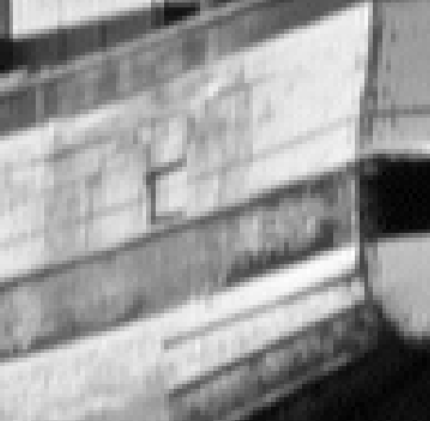
\includegraphics[width=\textwidth]{../report_images/boat_crop.png}
        \caption{Original Image}
      \end{subfigure}
      \hfill
      \begin{subfigure}[b]{0.4\textwidth}
        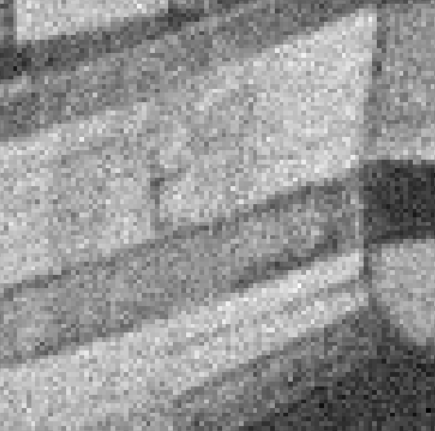
\includegraphics[width=\textwidth]{../report_images/noisy.png}
        \caption{Corrputed Image}
      \end{subfigure}
    \end{center}
  \end{figure}

  \newpage
  \begin{center}
    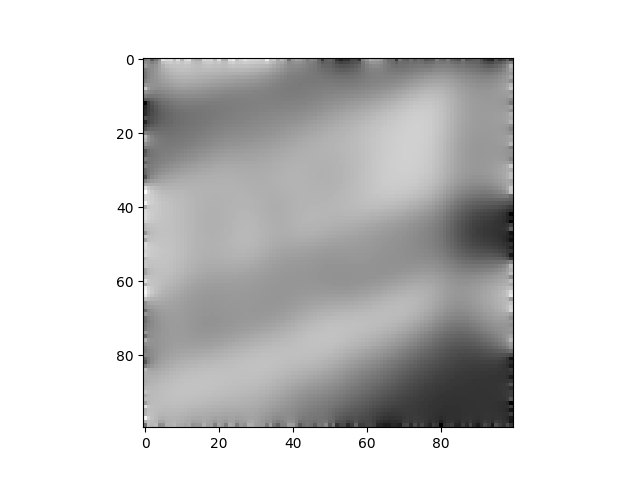
\includegraphics[width=\textwidth]{../generated_images/LinearHeat_test1.png}
    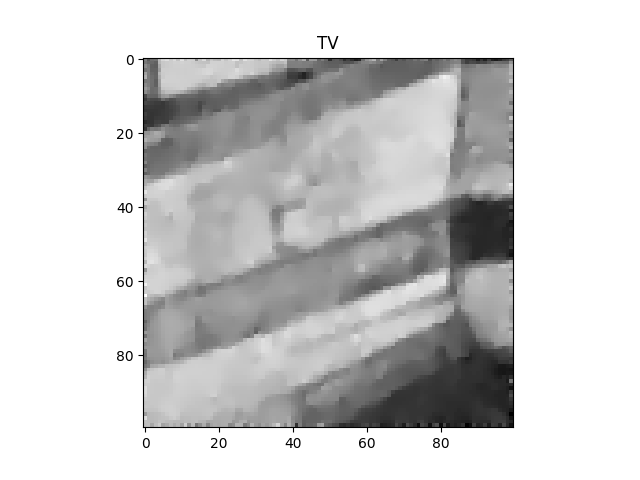
\includegraphics[width=\textwidth]{../generated_images/TV_test1.png}
  \end{center}

  %%%%%%%%%%%%%%%%%%%%%%%%%%%%%%
  % Experimental Results
  %%%%%%%%%%%%%%%%%%%%%%%%%%%%%%
  \newpage
  \subsection{Experimental Results}
  All results were generated by running the Evaluation.py script.\\

  %%%%%%%%%%%%%
  % Baseline
  %%%%%%%%%%%%%
  \noindent
  \textbf{1. Baseline Smoothing}\\
  In this test, the Custom PDE parameters are all set to one or zero to use 
  a penalty associated with a typical sigmoid.\\
  \begin{center}
    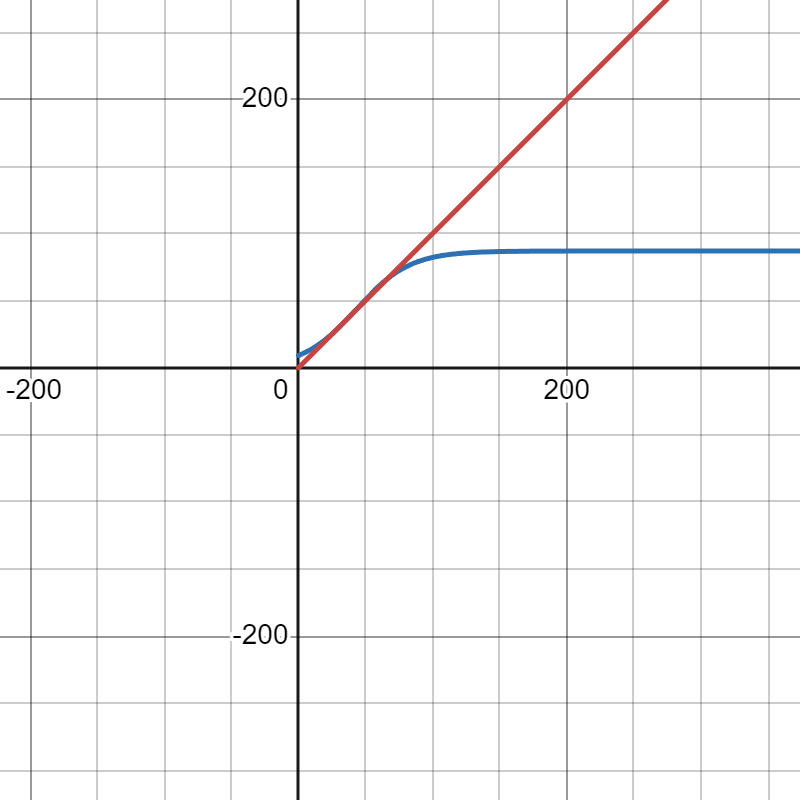
\includegraphics[scale=0.1]{../report_images/baseline_smoothing.png}\\
  \end{center}

  \noindent The mean square error is reduced more quickly for the sigmoidal penalty
  compared to the linear penalty, however the result still shows acceptable
  edge preservation characteristics.
  \begin{center}
    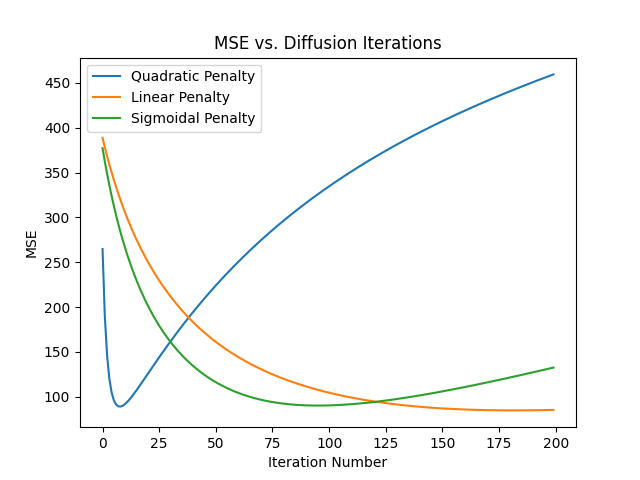
\includegraphics[scale=.5]{../generated_images/MSE_test1.png}\\
  \end{center}
  \begin{center}
    \begin{figure}[!htb]
      \begin{center}
        \begin{subfigure}[b]{0.3\textwidth}
          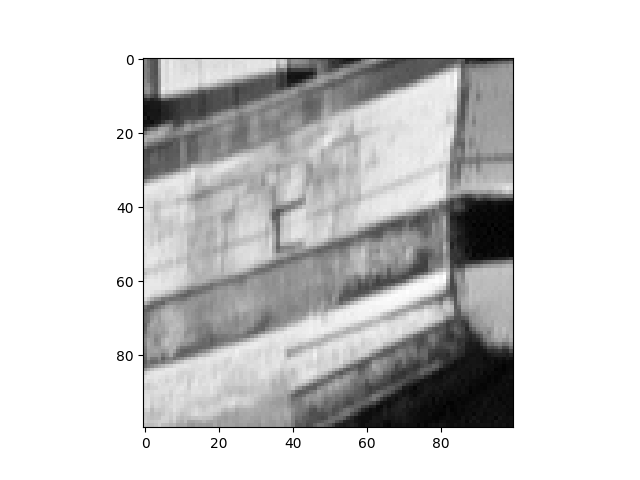
\includegraphics[width=\textwidth]{../report_images/boat_plot.png}
          \caption{Original Image}
        \end{subfigure}
        \hfill
        \begin{subfigure}[b]{0.3\textwidth}
          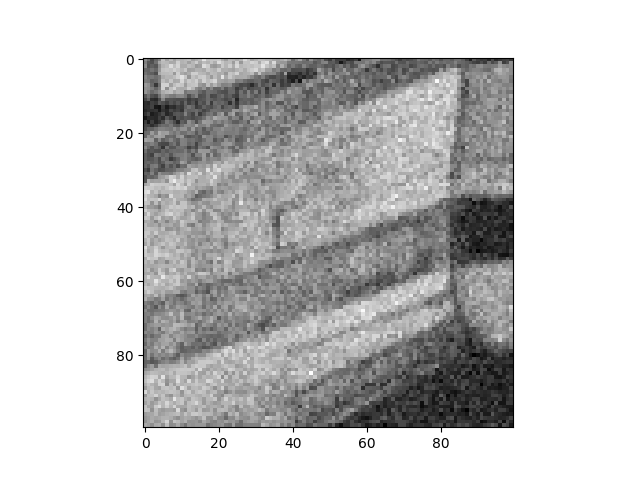
\includegraphics[width=\textwidth]{../report_images/noisy_boat_plot.png}
          \caption{Corrputed Image}
        \end{subfigure}
        \hfill
        \begin{subfigure}[b]{0.3\textwidth}
          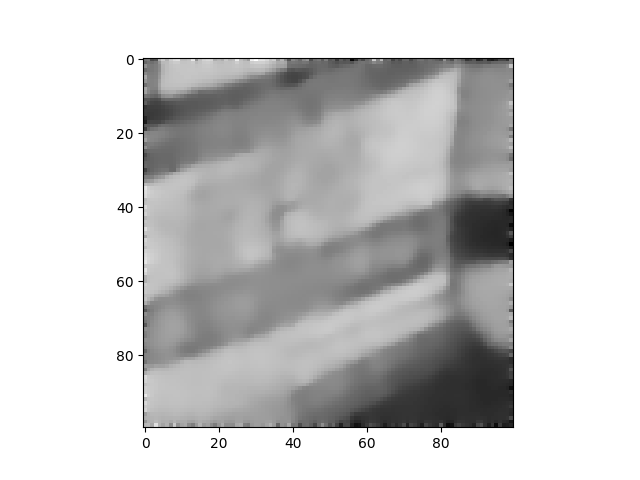
\includegraphics[width=\textwidth]{../generated_images/Custom_test1.png}
          \caption{Smoothed Image}
        \end{subfigure}
      \end{center}
    \end{figure}
  \end{center}

  %%%%%%%%%%%%%
  % Linear
  %%%%%%%%%%%%%
  \newpage
  \noindent
  \textbf{2. ``Linear'' Smoothing}\\
  In this test, the Custom PDE parameters are set such that the sigmoidal penalty
  traces the linear penalty before going flat.
  \begin{center}
    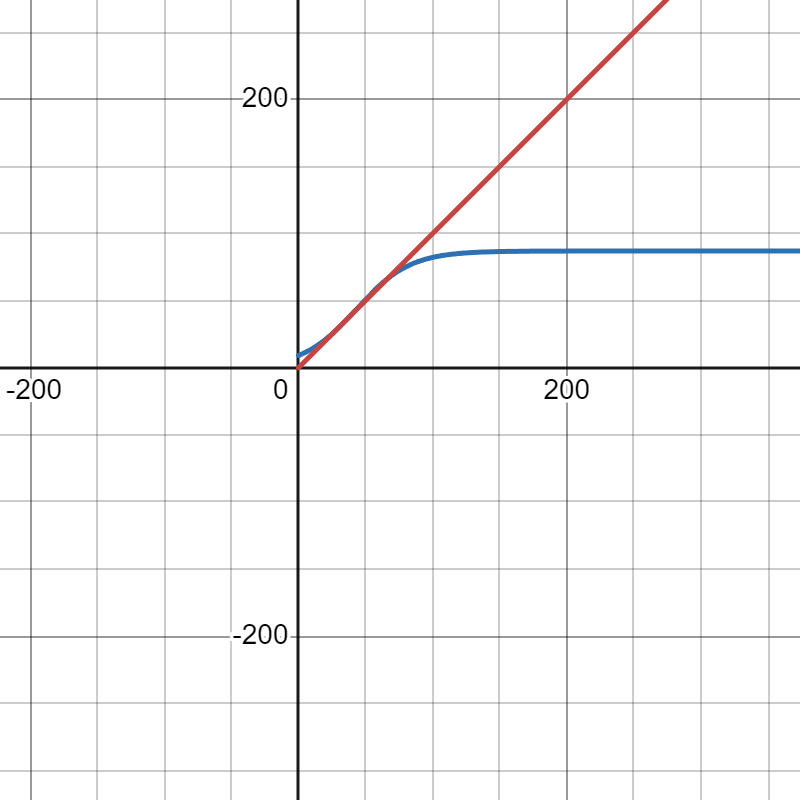
\includegraphics[scale=0.1]{../report_images/linear_smoothing.png}\\
  \end{center}

  \noindent 
  Compared to the previous test, we see that this image has a slightly
  more pronounced edge at the top of the center window. Additionally,
  the number of iterations required to reach the minimum MSE decreased.
  \begin{center}
    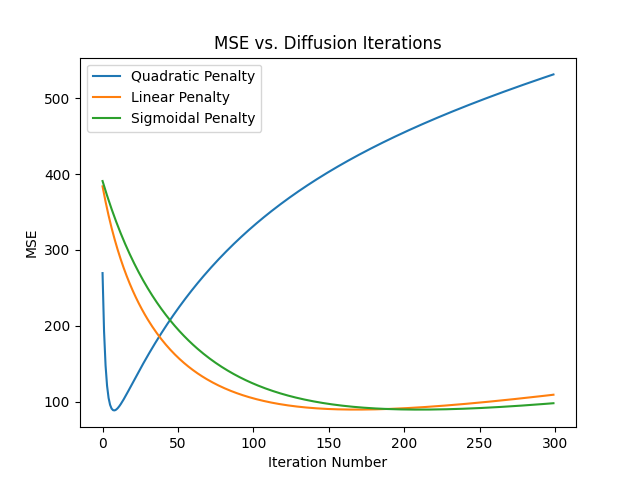
\includegraphics[scale=0.5]{../generated_images/MSE_test2.png}\\
  \end{center}
  \begin{center}
    \begin{figure}[!htb]
      \begin{center}
        \begin{subfigure}[b]{0.3\textwidth}
          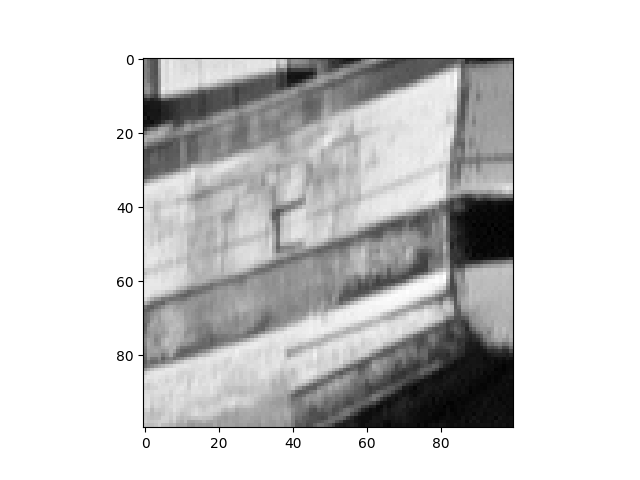
\includegraphics[width=\textwidth]{../report_images/boat_plot.png}
          \caption{Original Image}
        \end{subfigure}
        \hfill
        \begin{subfigure}[b]{0.3\textwidth}
          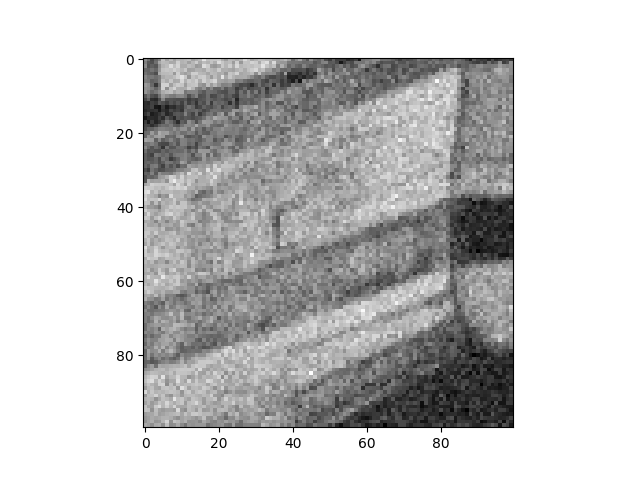
\includegraphics[width=\textwidth]{../report_images/noisy_boat_plot.png}
          \caption{Corrputed Image}
        \end{subfigure}
        \hfill
        \begin{subfigure}[b]{0.3\textwidth}
          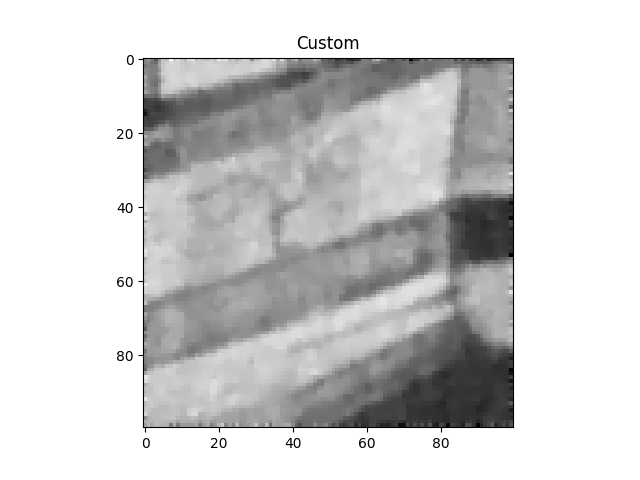
\includegraphics[width=\textwidth]{../generated_images/Custom_test2.png}
          \caption{Smoothed Image}
        \end{subfigure}
      \end{center}
    \end{figure}
  \end{center}

  %%%%%%%%%%%%%
  % Aggressive
  %%%%%%%%%%%%%
  \newpage
  \noindent
  \textbf{3. Aggressive Smoothing}\\
  Custom PDE slope matching linear penalty for range 10 to 75.\\
  \begin{center}
    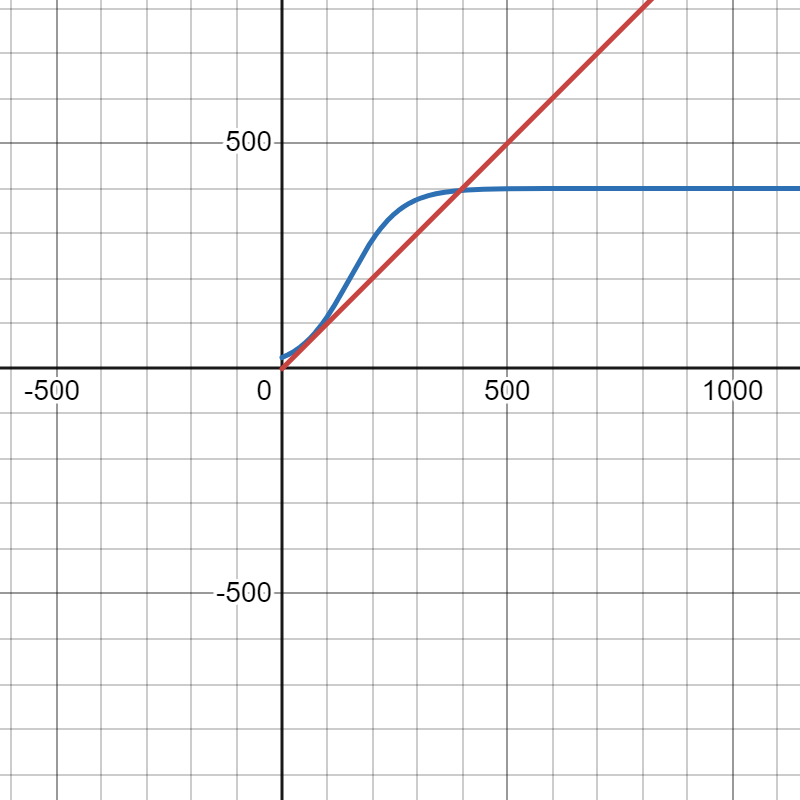
\includegraphics[scale=0.1]{../report_images/aggressive_smoothing.png}\\
  \end{center}

  \noindent The mean square error is reduced more quickly for the sigmoidal penalty
  compared to the linear penalty, however the result still shows acceptable
  edge preservation characteristics.
  \begin{center}
    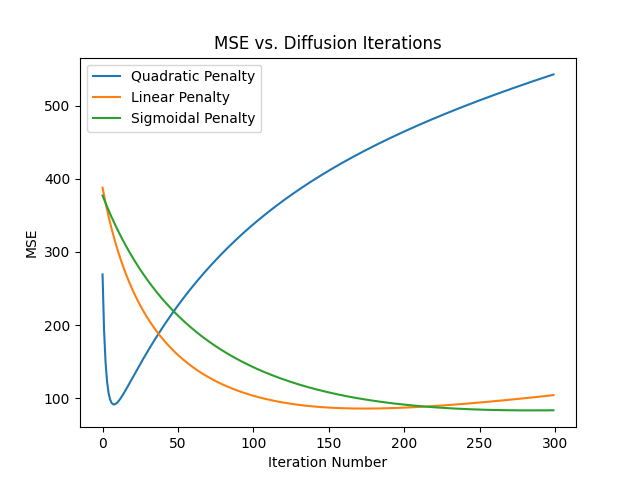
\includegraphics[scale=0.5]{../generated_images/MSE_test3.png}\\
  \end{center}
  \begin{center}
    \begin{figure}[!htb]
      \begin{center}
        \begin{subfigure}[b]{0.3\textwidth}
          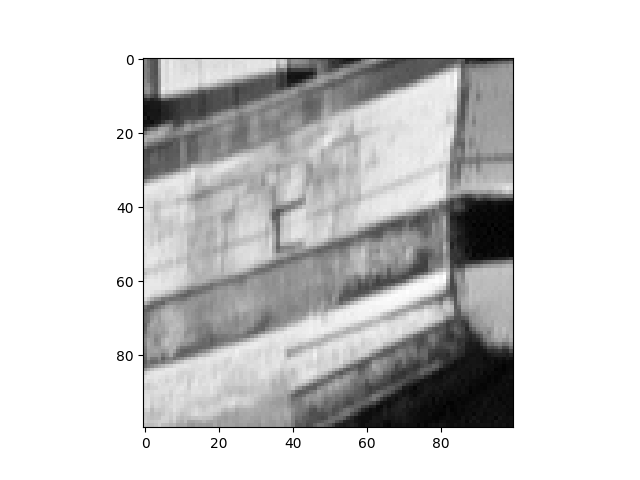
\includegraphics[width=\textwidth]{../report_images/boat_plot.png}
          \caption{Original Image}
        \end{subfigure}
        \hfill
        \begin{subfigure}[b]{0.3\textwidth}
          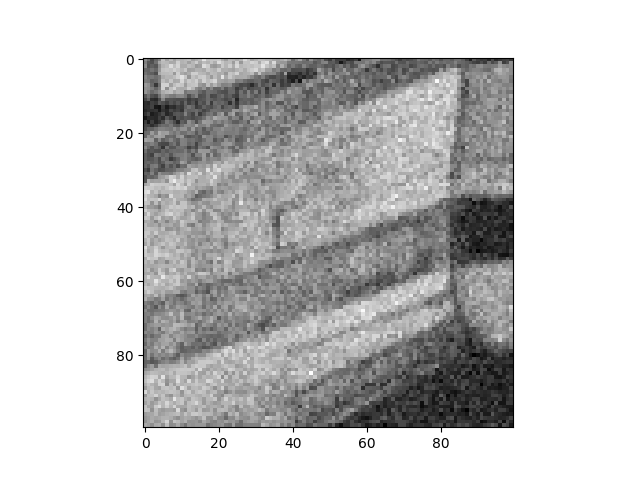
\includegraphics[width=\textwidth]{../report_images/noisy_boat_plot.png}
          \caption{Corrputed Image}
        \end{subfigure}
        \hfill
        \begin{subfigure}[b]{0.3\textwidth}
          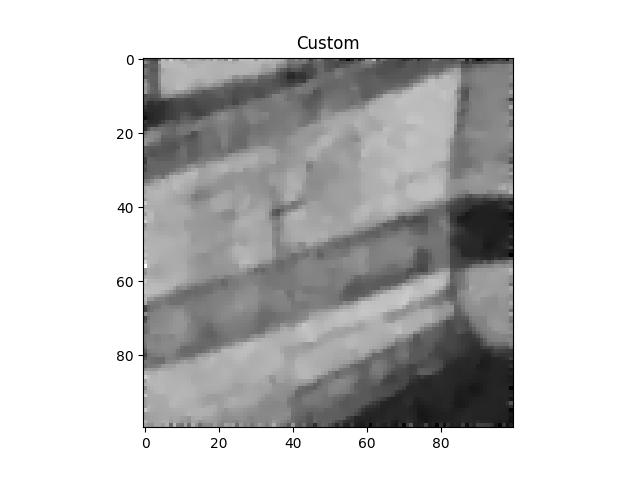
\includegraphics[width=\textwidth]{../generated_images/Custom_test3.png}
          \caption{Smoothed Image}
        \end{subfigure}
      \end{center}
    \end{figure}
  \end{center}

  %%%%%%%%%%%%%
  % Tempered
  %%%%%%%%%%%%%
  \newpage
  \noindent
  \textbf{4. Tempered Smoothing}\\
  Custom PDE slope matching linear penalty for range 10 to 75.\\
  \begin{center}
    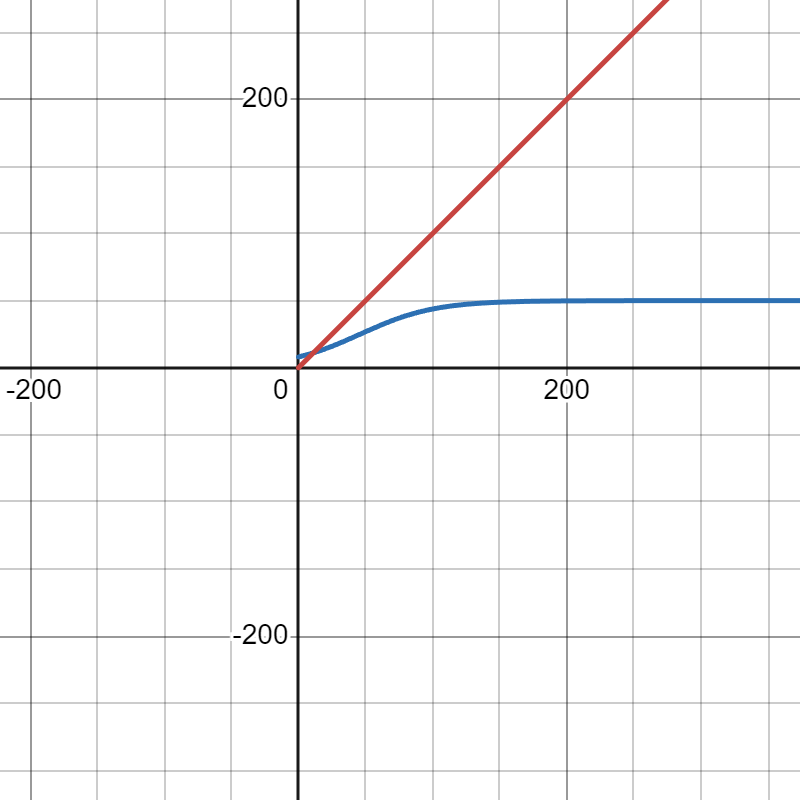
\includegraphics[scale=0.1]{../report_images/tempered_smoothing.png}\\
  \end{center}

  \noindent For this test the MSE plot seems to correspond to
  test (1). After reaching the its minimum, the MSE begins to
  increase at a rate less than what is seen in test (2) and (3).
  \begin{center}
    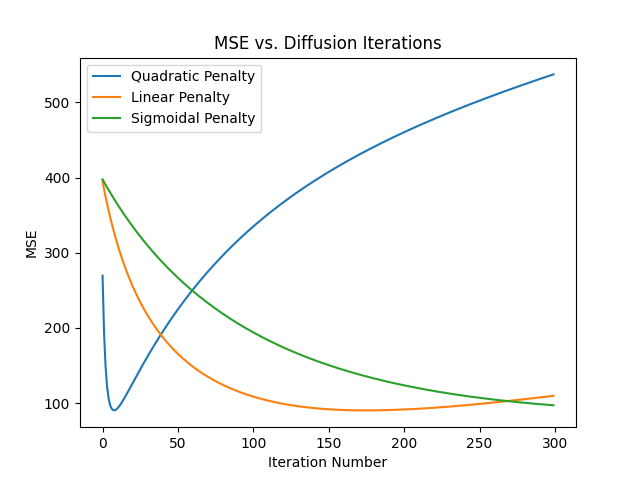
\includegraphics[scale=0.5]{../generated_images/MSE_test4.png}\\
  \end{center}
  \begin{center}
    \begin{figure}[!htb]
      \begin{center}
        \begin{subfigure}[b]{0.3\textwidth}
          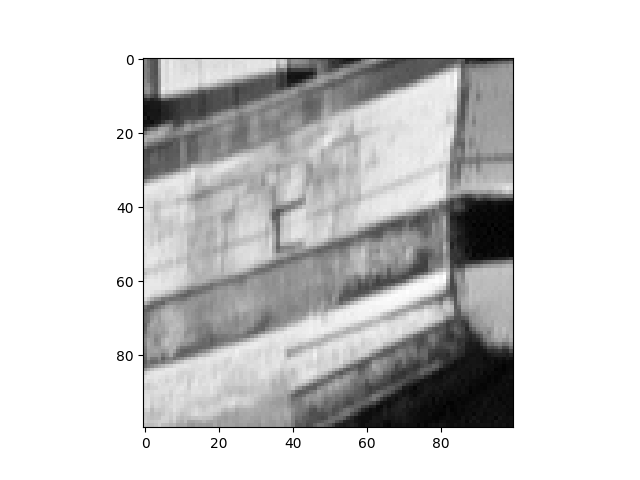
\includegraphics[width=\textwidth]{../report_images/boat_plot.png}
          \caption{Original Image}
        \end{subfigure}
        \hfill
        \begin{subfigure}[b]{0.3\textwidth}
          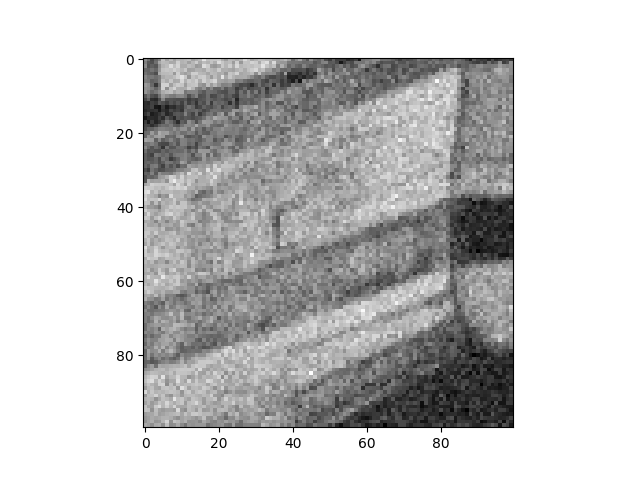
\includegraphics[width=\textwidth]{../report_images/noisy_boat_plot.png}
          \caption{Corrputed Image}
        \end{subfigure}
        \hfill
        \begin{subfigure}[b]{0.3\textwidth}
          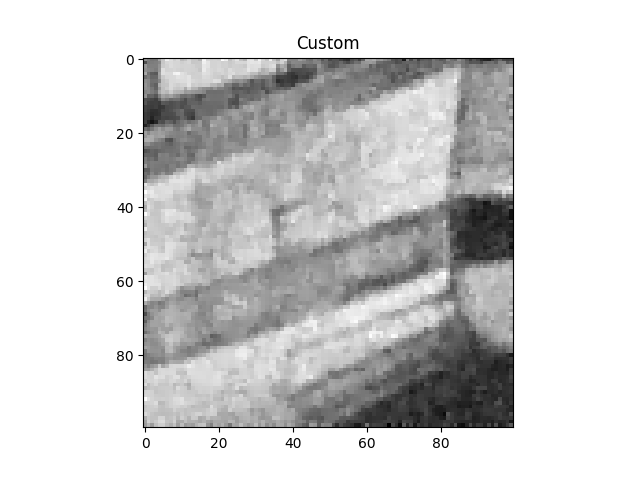
\includegraphics[width=\textwidth]{../generated_images/Custom_test4.png}
          \caption{Smoothed Image}
        \end{subfigure}
      \end{center}
    \end{figure}
  \end{center}

  %%%%%%%%%%%%%
  % MSE Table
  %%%%%%%%%%%%%
  \newpage
  \noindent
  \textbf{Minimum Computed MSE}
  \begin{table}[h]
    \begin{tabular}{|l|l|ll|lllll|}
    \hline
    Test Number & Linear Heat MSE & \multicolumn{2}{l|}{TV Diffusion MSE} & \multicolumn{5}{l|}{Sigmoidal MSE}  \\ \hline
    1           &  88.97          & \multicolumn{2}{l|}{84.67}            & \multicolumn{5}{l|}{90.05}          \\ \hline
    2           &  87.87          & \multicolumn{2}{l|}{89.72}            & \multicolumn{5}{l|}{91.19}          \\ \hline
    3           &                 & \multicolumn{2}{l|}{}                 & \multicolumn{5}{l|}{}               \\ \hline
    4           &  87.42          & \multicolumn{2}{l|}{91.10}            & \multicolumn{5}{l|}{87.52}          \\ \hline
    \end{tabular}
    \end{table}

  \vspace{12 pt}
  \noindent \textbf{Test 4 - Best smoothing result:}
  \begin{center}
    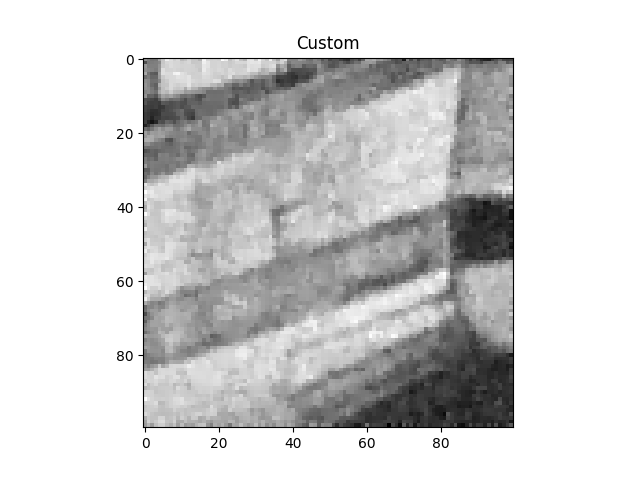
\includegraphics[width=\textwidth]{../generated_images/Custom_test4.png}
  \end{center}


  %%%%%%%%%%%%%%%%%%%%%%%%%%%%%%%%%%%%%%%%%%%%%%%%%%%%%%%%%%%%%%%
  % Conclusion
  %%%%%%%%%%%%%%%%%%%%%%%%%%%%%%%%%%%%%%%%%%%%%%%%%%%%%%%%%%%%%%%
  \newpage
  \section{Conclusion}

  \noindent
  The experiments showed that we were able to successfully
  denoise images using the custom PDE. From a qualitative
  perspective, the best smoothing result for the custom PDE
  has noticeably less blurring than the result obtained from smoothing via
  the Linear Heat equation. From a quantitative perspective, the
  collected data shows that the custom PDE was not able to
  significantly outperform the other methods.\\

  \noindent
  Despite not directly outperforming the other PDEs, the experiments did highlight some
  other potential advantages of the custom PDE.
  In all tests, the TV diffusion PDE and the custom PDE had equivalent values set for
  $\Delta t$ and $\epsilon$. Furthermore, in test 1, parameters $\lambda = 1$, $\beta=1$,
  and $c=0$ giving a penalty corresponding to a standard sigmoid function. The custom
  PDE was able to reach its minimum in far fewer iterations than the TV diffusion PDE.
  Although the current implementation of the custom PDE update is more computationally
  intensive than that of the TV diffusion PDE, for the 100x100 test image,
  each iteration saved is worth 10,000 pixels that do not need to be updated. Depending on the specific
  application, it may be advantageous to design a PDE in a certain way
  that considers both smoothing and computational performance.\\

  \noindent
  One challenge that arose while working with the custom PDE was deciding
  how to balance the various parameters including $\lambda$, $\beta$,
  $c$, etc. The selection of values for the parameters was performed
  heuristically in order to examine how the varying forms of the
  penalty function can impact smoothing performance. In the future,
  an option to sweep various parameters and observe the impact
  on a greater array of quality metrics could potentially lead to
  a selection of parameters that improve the performance
  of the PDE.\\

  \noindent
  Overall, this project showcased the powerful role PDEs can
  play in image processing. Previously, my perspective was limited
  to the idea that image smoothing is simply conducted via convolution
  and that the smoothing can only be paid for by accepting
  blurring to the image. Instead, smoothing can be thought of 
  as an iterative diffusion process. The designer of the
  PDE is able to control how the smoothing effect will
  behave in different regions of an image.


  %%%%%%%%%%%%%%%%%%%%%%%%%%%%%%%%%%%%%%%%%%%%%%%%%%%%%%%%%%%%%%%
  % References
  %%%%%%%%%%%%%%%%%%%%%%%%%%%%%%%%%%%%%%%%%%%%%%%%%%%%%%%%%%%%%%%
  \newpage
  \urlstyle{same}
  \section{References}
  \begin{enumerate}
    \item \url{https://web.archive.org/web/20060718054020/http://www.acm.uiuc.edu/siggraph/workshops/wjarosz_convolution_2001.pdf}
    \item \url{https://www.mia.uni-saarland.de/weickert/Papers/book.pdf}
    \item \url{https://www.uni-muenster.de/Physik.TP/archive/fileadmin/lehre/part2_hypebolic/node7.html}
  \end{enumerate}

\end{document}